\chapter[Metodologia]{Metodologia}

Este capítulo apresenta a metodologia utilizada, que se trata de como o trabalho foi desenvolvido, visando responder às questões elaboradas na introdução.

A metodologia selecionada foi a Revisão Sistemática de Literatura (RSL). Trata-se de uma abordagem rigorosa para identificar, avaliar e sintetizar evidências relevantes sobre uma questão específica de pesquisa. É um método amplamente utilizado em muitas áreas para fixar o entendimento sobre algum tema em específico e direcionar pesquisas futuras. A RSL é um estudo secundário, pois é baseado em estudos primários que já foram publicados.

Neste trabalho, adotou-se uma versão abreviada da RSL devido às limitações de tempo do Trabalho de Conclusão de Curso (TCC). A aplicação completa da metodologia demandaria um período mais extenso para sua execução, o que tornaria inviável sua realização dentro do escopo deste estudo.

Para conduzir uma RSL de maneira estruturada e eficiente, o processo é dividido em três fases principais: o \textbf{planejamento}, a \textbf{condução} e os \textbf{resultados}. Logo abaixo, segue um diagrama com as etapas desta RSL.

\begin{figure}[h]
	\centering % para centralizarmos a figura
	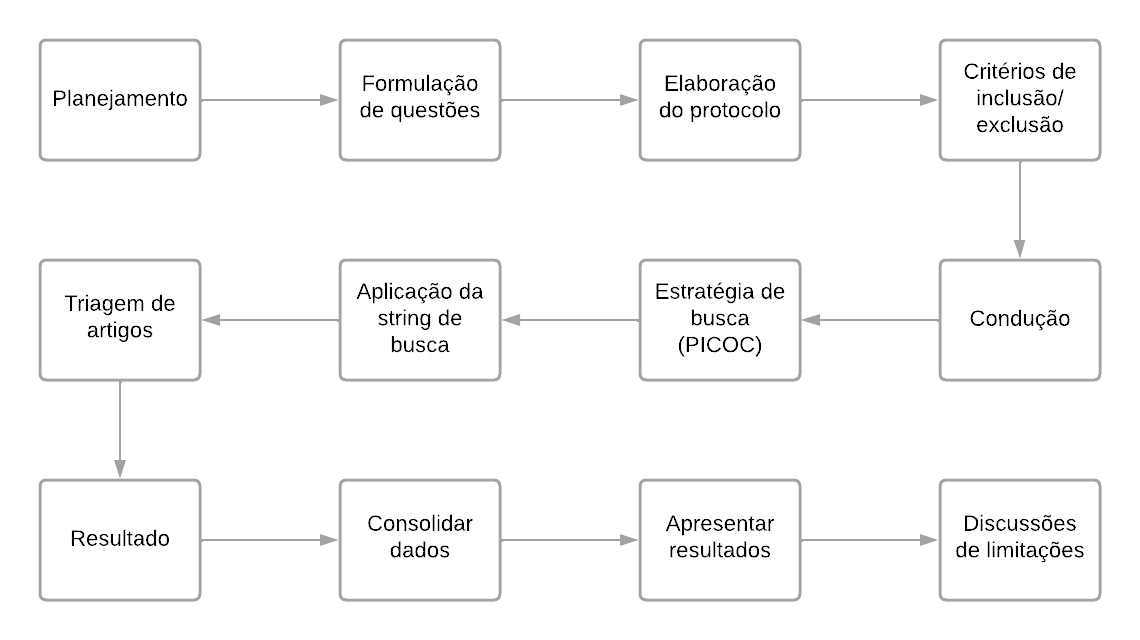
\includegraphics[width=16cm]{figuras/diagrama-RSL.png} % leia abaixo
	\caption{Etapas da RSL}
	Fonte: Elaboração própria
	\label{figura:diagrama rsl}
\end{figure}

\begin{itemize}
	\item \textbf{Planejamento}

A fase de planejamento é crucial para a organização da RSL. O objetivo desta etapa é identificar a necessidade de realizar a revisão e definir de maneira clara os objetivos. Isso inclui duas atividades-chave, sendo elas:

	\begin{itemize}
		\item 
		\textbf{Formular as questões de pesquisa}
		
			As questões de pesquisa são essenciais para guiar todo o processo de busca e análise na RSL. Elas devem ser formuladas de maneira clara e objetiva, alinhando-se aos objetivos do estudo e ao escopo da revisão, para que os estudos selecionados sejam pertinentes e as evidências encontradas possam responder diretamente às perguntas propostas. Além disso, as questões de pesquisa devem ser formuladas com base nas lacunas de conhecimento identificadas no tema, e podem ser ajustadas ao longo do processo, conforme necessário, para garantir que a revisão aborde de forma eficaz os aspectos mais relevantes do problema de pesquisa.
		
		\item 
		\textbf{Elaboração do protocolo}
		
			 Descreve os critérios de inclusão e exclusão de estudos. Além disso, define quais serão as fontes de dados a serem utilizadas (como bases de dados eletrônicas, livros, anais de conferências e outras publicações relevantes). Por último, mas não menos importante, os procedimentos para coleta e organização das informações. Esse protocolo serve como um guia para toda a RSL.
	\end{itemize}

	\item \textbf{Condução}
	
	Esta etapa é a fase operativa da RSL, onde a estratégia de busca definida anteriormente é colocada em prática. Essa estratégia pode incluir combinações de palavras-chave, operadores lógicos e filtros específicos que permitam localizar os estudos mais relevantes para a pesquisa nas fontes selecionadas. Uma vez coletados, os estudos passam por uma triagem baseada nos critérios de inclusão e exclusão estabelecidos no protocolo, para assim, filtrar ainda mais os estudos.
	
	Logo após, é realizada uma análise crítica do conteúdo dos estudos selecionados, com o objetivo de extrair e organizar as informações relevantes. A principal finalidade dessa fase é responder às questões de pesquisa propostas, garantindo que a resposta tenha como base as evidências obtidas a partir dos estudos.
	
	\item \textbf{Resultado}
	
	Esta é a fase final da RSL, que é dedicada à documentação e apresentação dos resultados. Aqui, os dados extraídos e analisados são consolidados em um relatório ou artigo científico, que inclui a descrição detalhada dos procedimentos adotados, as evidências encontradas e as respostas às questões de pesquisa. Esta fase também pode envolver a elaboração de tabelas, gráficos e diagramas que auxiliem na compreensão dos resultados.
	
	É importante destacar que os achados da RSL devem ser interpretados considerando-se suas limitações, como possíveis vieses nos estudos primários ou na seleção dos mesmos.
	
\end{itemize}

\section{Planejamento}

\subsection{Questões de pesquisa}

Para elaboração das questões de pesquisa, os objetivos deste trabalho foram utilizados como base principal. As questões 1, 2 e 3 estão ligadas ao primeiro objetivo específico, as questões 4 e 5 estão ligadas ao segundo objetivo específico e a questão 6 está ligada ao terceiro objetivo específico. Como resultado, estão listadas abaixo as questões de pesquisa.

%Talvez fazer uma tabela relacionando cada questão com seu objetivo específico relativo

\begin{enumerate}
	
	\item Quais são as principais técnicas de prototipação utilizadas no Design de Serviços (DS)?
	\item Como essas técnicas são caracterizadas em termos de objetivos, métodos e resultados esperados?
	\item Em quais contextos ou etapas do DS essas técnicas são mais aplicáveis?
	
	\item Quais ferramentas de prototipação são mais utilizadas no DS?
	\item Como essas ferramentas se comparam em termos de funcionalidades e adequação às diferentes etapas do processo de DS?
	
	\item Quais são as entradas necessárias e as saídas esperadas no processo de prototipação em DS?
	
\end{enumerate}

\subsection{Estratégia de busca}

A estratégia de busca dessa RSL foi elaborada utilizando como base o modelo População, Intervenção, Comparação, Resultado e Contexto (PICOC). Este modelo fornece uma estrutura lógica para a definição de critérios de busca. Logo abaixo, cada elemento do PICOC é descrito em relação ao tema do trabalho.

\begin{itemize}
	\item \textbf{População (P)}
	
	Define o grupo de interesse relacionado ao tema do estudo.
	
	Neste estudo, a população abrange estudos relacionados ao DS.
	\begin{itemize}
		\item Palavras-chave: \textit{``Service Design'', ``Service Development''}.
	\end{itemize}
	
	\item \textbf{Intervenção (I)}
	
	Estabelece as ações, técnicas ou ferramentas que estão sendo investigadas.
	
	Neste estudo, a intervenção está relacionada à \textbf{prototipação}, incluindo técnicas e ferramentas utilizadas nesse contexto.
	
	\begin{itemize}
		\item Palavras-chave: \textit{``Prototyping'', ``Prototyping Techniques'', ``Prototyping Tools''}.
	\end{itemize}
	
	\item \textbf{Comparação (C)}
	
	Especifica se haverá alguma comparação explícita entre alternativas.
	
	Neste estudo não haverá nenhuma comparação obrigatória, porém alguns estudos podem acabar comparando diferentes técnicas ou ferramentas de prototipação. 
	
	\item \textbf{Resultado (O)}
	
	Indica os resultados esperados.
	
	Neste estudo, os resultados esperados incluem a identificação de ferramentas de prototipação, informações sobre entradas e saídas do processo e sua interação com outras etapas do desenvolvimento.
	
	\begin{itemize}
		\item Palavras-chave:\textit{ ``Effectiveness'', ``Outcomes'', ``Results'', ``Impact''}.
	\end{itemize} 
	
	\item \textbf{Contexto (C)}
	%Repensar o contexto, talvez usar o contexto de prototipação para resultados mais abrangentes.
	
	Estabelece o cenário em que o estudo foi realizado.
	Neste estudo, o contexto inclui estudos que abordem prototipação em geral, além do DS. Os estudos selecionados devem obrigatoriamente abordar ao menos um dos dois temas.
	
	\begin{itemize}
		\item Palavras-chave: \textit{``Prototyping Process'', ``Prototyping Applications'', ``Service Design'', ``Service Prototyping'', ``Service Development''}.
	\end{itemize}
	
\end{itemize}

\subsection{\textit{String} de busca}

Com base nos elementos do modelo PICOC, principalmente nas palavras-chave, uma \textit{string} de busca foi desenvolvida utilizando operadores booleanos (\textit{AND}, \textit{OR}) para combinar os termos identificados e realizar a busca pelos estudos nas bases de dados definidas. A \textit{string} foi adaptada para cada base de dados utilizada, visando respeitar suas especificidades. Logo abaixo, a \textit{string} base é apresentada:

( (\textit{ ``prototyping'' OR ``prototyping techniques'' OR ``prototyping tools'' OR ``prototyping process'' ) AND ( ``process'' OR ``methods'' OR ``outcomes'' OR ``results'' ) AND ( ``service design'' OR ``service prototyping'' OR ``service development''}) )

%( (prototyping OR "prototyping techniques" OR "prototyping tools" OR "prototyping process") AND (process OR methods OR outcomes OR results) AND ("service design" OR "service prototyping" OR "service development") )

\subsection{Bases de dados}

Para a escolha das bases de dados, o principal critério levado em consideração foi a relevância da base, para garantir que o trabalho esteja alinhado com os estudos mais relevantes. Como resultado, as bases selecionadas foram a \textbf{\textit{Scopus}}, \textbf{Coordenação de Aperfeiçoamento de Pessoal de Nível Superior (CAPES)}, \textbf{\textit{ACM Digital Library}, \textbf{\textit{ScienceDirect}} e \textbf{\textit{Springer}}}.

\subsection{Critérios de seleção}

Para realizar uma triagem primária, alguns critérios de inclusão e exclusão foram elaborados.

Critérios de inclusão:
\begin{itemize}
	\item O trabalho deve ter sido publicado após o ano de 2021.
	
	\item O trabalho deve estar disponível nas bases de dados previamente definidas.
	
	\item O estudo deve ter sido escrito em inglês ou português.
	
\end{itemize}

Como critérios de exclusão, considera-se, além do não obedecimento dos critérios de inclusão, os seguintes critérios:
\begin{itemize}
	\item Trabalho com acesso pago.
\end{itemize}

\section{Condução}

Com o planejamento finalizado, o próximo passo foi a realização da condução da revisão.

\subsection{Procedimentos de seleção}

O procedimento de seleção dos artigos para o estudo obedeceu uma sequência de passos. Esses passos serviram como uma triagem para a seleção dos artigos mais relevantes para compor o estudo. Logo abaixo estão os passos para a seleção dos artigos, assim como uma tabela indicando o número de artigos selecionados após a execução de cada passo.

\begin{enumerate}
	\item Aplicação da \textit{string} de busca nas bases selecionadas. %Com isso, uma lista provisória de artigos foi gerada.
	
	\item Aplicação dos critérios de inclusão e exclusão. %Neste momento foi possível realizar o descarte dos artigos que não obedeciam os critérios previamente estabelecidos.
	
	\item Remoção dos artigos duplicados. %Como a busca foi realizada em duas bases, os artigos duplicados foram removidos.
	
	\item Leitura do título e resumo dos artigos. %Aqui, foi possível realizar o descarte de artigos que não fazem muito sentido para o objetivo do estudo.
	
	\item Leitura do artigo. %Assim, é garantida a relevância do mesmo para o etudo.
\end{enumerate} 

\begin{table}[h!]
	\centering
	\label{tab:triagem}
	\begin{tabular}{|c|c|c|c|c|c|c|}
		\hline
		\textbf{Passo} & \textbf{Scopus} & \textbf{CAPES} & \textbf{ACM} & \textbf{ScienceDirect} & \textbf{Springer} & \textbf{Total} \\ \hline
		1 & 156 & 602 & 1146 & 2224 & 1675 & 5803\\ \hline
		2 & 39 & 125 & 362 & 712 & 106 & 1344\\ \hline
		3 & 39 & 85 & 362 & 712 & 106 & 1304\\ \hline
		4 & 10 & 11 & 39 & 41 & 20 & 121\\ \hline
		5 & 7 & 7 & 3 & 5 & 3 & 25 \\ \hline
	\end{tabular}
	\caption{Quantidade de artigos após cada passo da triagem nas bases}
\end{table}


\subsection{Seleção de estudos primários}

O processo de seleção de estudos primários foi iniciado através da pesquisa utilizando a \textit{string} de busca nas bases digitais selecionadas. A busca automática nas bases escolhidas gerou um total de 5803 artigos.

Logo após, os critérios de inclusão e exclusão foram aplicados, excluindo os artigos que não obedeciam todos os critérios. A aplicação dos critérios de inclusão e exclusão resultou em um total de 1344 artigos.

Em seguida, como a pesquisa foi feita em duas bases, os artigos duplicados foram removidos. A remoção dos artigos duplicados resultou em um total de 1304 artigos.

Na sequência, a leitura do título e resumo dos artigos permitiu realizar o descarte de artigos que ainda sim não respondiam nenhuma das questões de pesquisa. A leitura do título e resumo dos artigos resultou em um total de 121 artigos.

Por último, a leitura dos artigos restantes garantiu que somente os artigos que eram relevantes para o contexto do estudo fossem selecionados. A leitura dos artigos resultou em um total de 27 artigos.

\subsection{Extração de dados}

A extração de dados se faz necessária para obtenção de informações pertinentes ao estudo. Ela foi iniciada com a exportação dos arquivos referentes aos artigos no formato BibTex. Esses arquivos, detinham informações essenciais para o estudo, como: título, autores, ano de publicação, número de paginas e resumo.

Conforme o andamento do trabalho, se fez necessário o download dos artigos por completo, a ferramenta Zotero foi utilizada para auxiliar nessa manipulação de dados.

\section{Resultado}

Após a realização da toda a condução da revisão, a quantidade de artigos, que inicialmente era de 758 artigos passou para 14 artigos. Com isso, a tabela abaixo lista os 14 artigos que passaram por todos os passos da triagem, identificando-os por um ID, autor/referência com ano de publicação e uma breve descrição. 

\begin{longtable}{|c|m{4cm}|m{10cm}|}
	\caption{Estudos utilizados na RSL} \label{tab:estudos} \\
	\hline
	\makecell{\textbf{ID}} & \makecell{\textbf{Autor, Referência}} & \makecell{\textbf{Descrição}} \\
	\hline
	\endfirsthead
	
	\multicolumn{3}{c}{\textit{Continuação da Tabela~\ref{tab:estudos}}} \\
	\hline
	\makecell{\textbf{ID}} & \makecell{\textbf{Autor, Referência}} & \makecell{\textbf{Descrição}} \\
	\hline
	\endhead
	
	\hline \multicolumn{3}{|r|}{Continua na próxima página} \\
	\hline
	\endfoot
	
	\hline
	\endlastfoot
	
	% Dados da tabela
	E1  & \cite{asbjornsen2022echange} & Descreve uma intervenção digital centrada no usuário para mudança de comportamento, combinando design thinking, agile e prototipação. \\ \hline
	E2  & \cite{dehmel2021weather} & Descreve um estudo de DS combinado com experimentos de escolha discreta, usando prototipação e métodos iterativos. \\ \hline
	E3  & \cite{giraldo2024ecotourism} & Explora o uso de DS e prototipação para criar experiências de realidade aumentada (AR) em PMEs de ecoturismo. \\ \hline
	E4  & \cite{kumar2023rheumatology} & Aplica o design thinking com prototipação para inovar entrevistas virtuais em reumatologia, centrando-se na experiência do candidato. \\ \hline
	E5  & \cite{lambe2022capabilities} & Aplica DS com mapeamento de experiência e prototipação para criar intervenções sustentáveis em comunidades de baixa renda. \\ \hline
	E6  & \cite{lee2023industry} & Explora o uso da prototipação no DS para criar novas soluções e melhorar a comunicação em projetos da Indústria 4.0, como o tratamento de águas residuais. \\ \hline
	E7  & \cite{milton2021eatingdisorders} & Destaca o uso do design participativo e prototipação para criar soluções tecnológicas no tratamento de distúrbios alimentares e imagem corporal. \\ \hline
	E8  & \cite{seko2024transitions} & Uso do design participativo para co-criar um modelo de serviço de transição para jovens com deficiência, aplicando prototipação. \\ \hline
	E9  & \cite{soto2023prototyping} & Explora como a prototipação de serviços, com foco na empatia, pode melhorar a experiência do usuário e aprimorar a pesquisa colaborativa no design de serviços. \\ \hline
	E10 & \cite{villa2022integratedcare} & Descreve o desenvolvimento de uma plataforma digital de cuidados personalizados para idosos, com prototipação e desenvolvimento ágil centrado no usuário. \\ \hline
	E11 & \cite{wang2023smartproducts} & Investiga as preferências de prototipação no design de produtos inteligentes, focando na comunicação entre disciplinas. \\ \hline
	E12 & \cite{yan2022pssvalue} & Explora como a prototipação pode transformar a estratégia PSS e melhorar o DS digitais em uma empresa automobilística. \\ \hline
	E13 & \cite{Kim2024} & Apresenta um framework educacional para capacitar estudantes de design, sem formação técnica, a desenvolver protótipos de IoT. \\ \hline
	E14 & \cite{Suryawati2024} & Desenvolveu uma plataforma web para tornar o aconselhamento escolar mais interativo, validada com alta pontuação de especialistas e usuários. \\ \hline
	E15 & \cite{hegemann2024palette} & Analisou a escolha de cores em design de serviço e prototipação via entrevistas. Propôs o framework purpose-palette-prototype e ferramentas para integração das etapas. \\ \hline
	E16 & \cite{lee2022how} & Analisou a adoção de design de serviço no HCI via revisão sistemática (179 artigos). Principais achados: foco em nível de interação (vs. sistêmico) e oportunidades futuras para integração de dimensões sistêmicas do design de serviço em HCI. \\ \hline
	E17 & \cite{quintero2021interdisciplinary} & Descreve o desenvolvimento de uma órtese assistiva via*co-design interdisciplinar e prototipação centrada em valores, integrando abordagem biopsicossocial no design de serviço. \\ \hline
	E18 & \cite{iriarte2023service} &Analisou o impacto do DS na servitização digital (Indústria 4.0) via estudo multicaso com 10 fabricantes. Destacou contribuições para proposição de valor de serviços avançados e processos iterativos de prototipação em design. \\ \hline
	E19 & \cite{leinonen2023service} & Mapeou a transferência de conhecimento entre DS e UX ágil via revisão sistemática (41 artigos). Proposição de frameworks e boas práticas para comunicação eficaz em projetos com processos iterativos e implementação ágil. \\ \hline
	E20 & \cite{mager2023product} & Propôs framework educacional para DS em sistemas produto-serviço, com ênfase em abordagens humanocentradas, ecossistêmicas e processos iterativos para evolução de sistemas complexos. \\ \hline
	E21 & \cite{nguyen2022human} & Propôs a metodologia DIMAND para DS avançado, integrando ciclo de vida, redes de stakeholders e processos iterativos via validação com especialistas. Abordagem humanocentrada aplicada à prototipação de serviços complexos. \\ \hline
	E22 & \cite{paust2025integrative} & Analisou o papel da prototipação em gestão via revisão integrativa. Definiu o conceito com foco em representação e interação com stakeholders, propondo agenda de pesquisa para integração de temas fragmentados. \\ \hline
	E23 & \cite{Vieira2025} & Propos integração de DS e desenvolvimento de novos serviços (NSD) via modelo híbrido (waterfall-cíclico), com processos iterativos e participação ativa do cliente para cocriação de valor e integração departamental. \\ \hline
	E24 & \cite{schlott2024design} & Analisou o impacto do design thinking no trabalho em equipe via revisão sistemática. Principais achados: influência em interações, habilidades e cultura organizacional, com implicações para processos iterativos em design de serviços. \\ \hline
	E25 & \cite{you2022applying} & Analisou a aplicação do design thinking em inovação de modelos de negócio via revisão crítica. Identificou sete temas-chave, incluindo co-criação e processos sociais, destacando sinergias com DS e processos iterativos de inovação. \\ \hline
	
\end{longtable}

%Agora, essas próximas etapas só serão realizadas no TCC 2, após a leitura e interpretação por completa dos artigos selecionados.

%\subsection{QP.1. Quais são as principais técnicas de prototipação utilizadas no Design de Serviços?}

%\subsection{QP.2. Como essas técnicas são caracterizadas em termos de objetivos, métodos e resultados esperados?}

%\subsection{QP.3. Em quais contextos ou etapas do Design de Serviços essas técnicas são mais aplicáveis?}

%\subsection{QP.4. Quais ferramentas de prototipação são mais utilizadas no Design de Serviços?}


%\subsection{QP.5. Como essas ferramentas se comparam em termos de funcionalidades e adequação às diferentes etapas do processo de Design de Serviços?}


%\subsection{QP.6. Quais são as entradas necessárias e as saídas esperadas no processo de prototipação em Design de Serviços?}

 
